\section{Lecture 14: Quantum Harmonic Oscillator, Dirac Notation}

Recall that from last lecture, we found the general wavefunction as:
\[ \Psi_n(\xi) = e^{-\epsilon^2/2} H_n(\xi) \]
where $\xi = \alpha x$, $\alpha = \qty(\frac{m\omega}{\hbar})^{1/2}$ and $H_n$ is the $n$th Hermite polynomial.
There are two ways to get these polynomials: either use a table or a generating function.
Here are the first few:
\begin{align*}
    H_0(\xi) &= 1 \\
    H_1(\xi) &= 2\xi \\
    H_2(\xi) &= 4\xi^2 - 2 \\
    H_3(\xi) &= 8\xi^3 - 12 \xi \\
    H_4(\xi) &= 16\xi^4 - 48\xi^2 + 12 \\
    &\vdots \\
    H_n(\xi) &= (-1)^n e^{\xi^2} \derivative{^n e^{-\xi^2}}{\xi^n} \\
    &= e^{\xi^2/2} \qty(\xi - \derivative{}{\xi})^n e^{-\xi^2/2}
\end{align*}

This means the wave function is:
\[ \Psi_n(x) = \qty(\frac{\alpha}{\sqrt{\pi} 2^n n!})^{1/2} e^{-\alpha^2 x^2/2} H_n(\alpha x) \]
with $E_n = \qty(n + 1/2) \hbar \omega$ (as we remember from last time).

This is what they look like, marking the ``classical turning points'' of a particle as ctp:

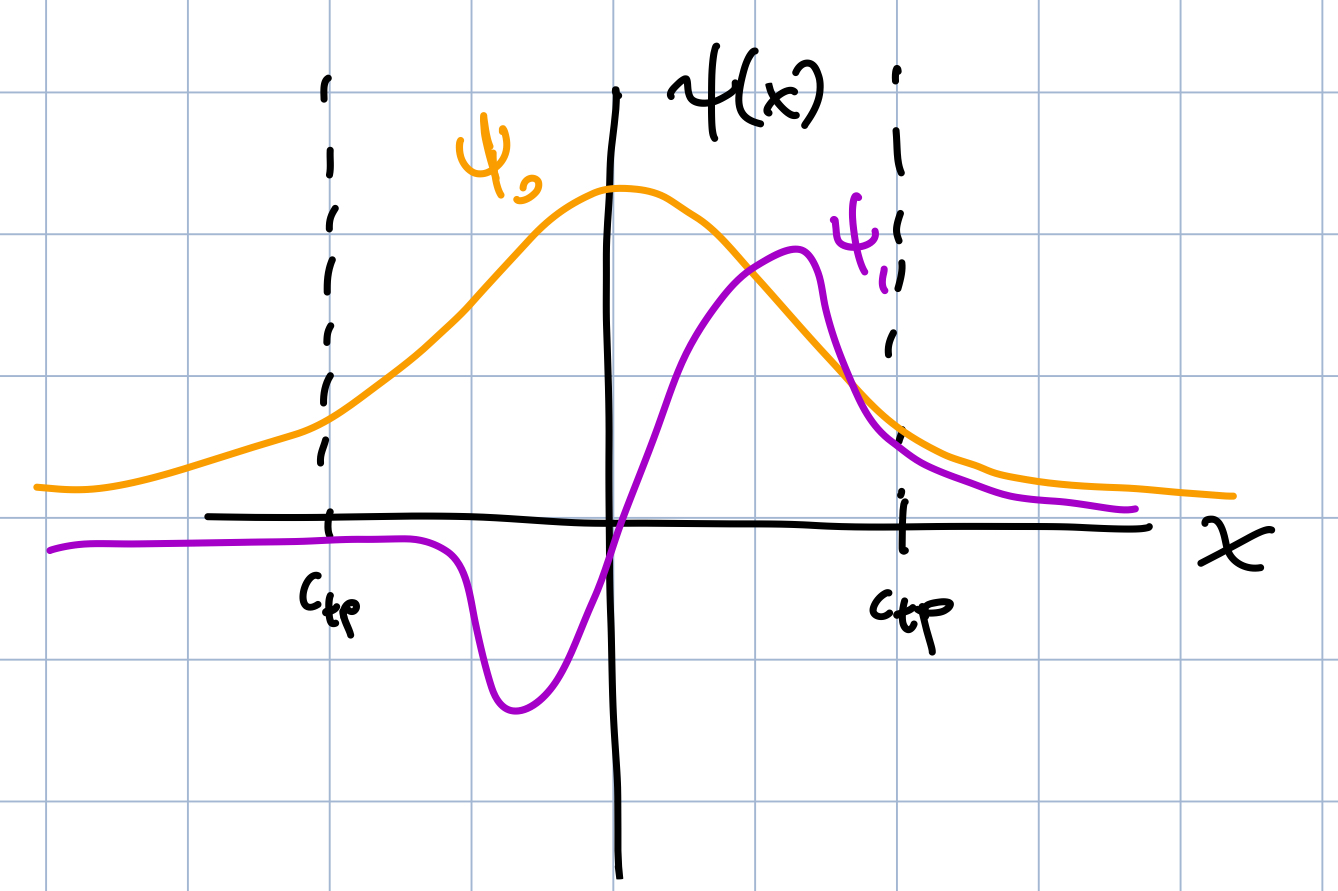
\includegraphics[width=300px]{mewhenimqhm.jpeg}

In a classical setting, a particle in an oscillator will spend most of its time near the ends. But
the probability density of a high-energy wave looks like this:

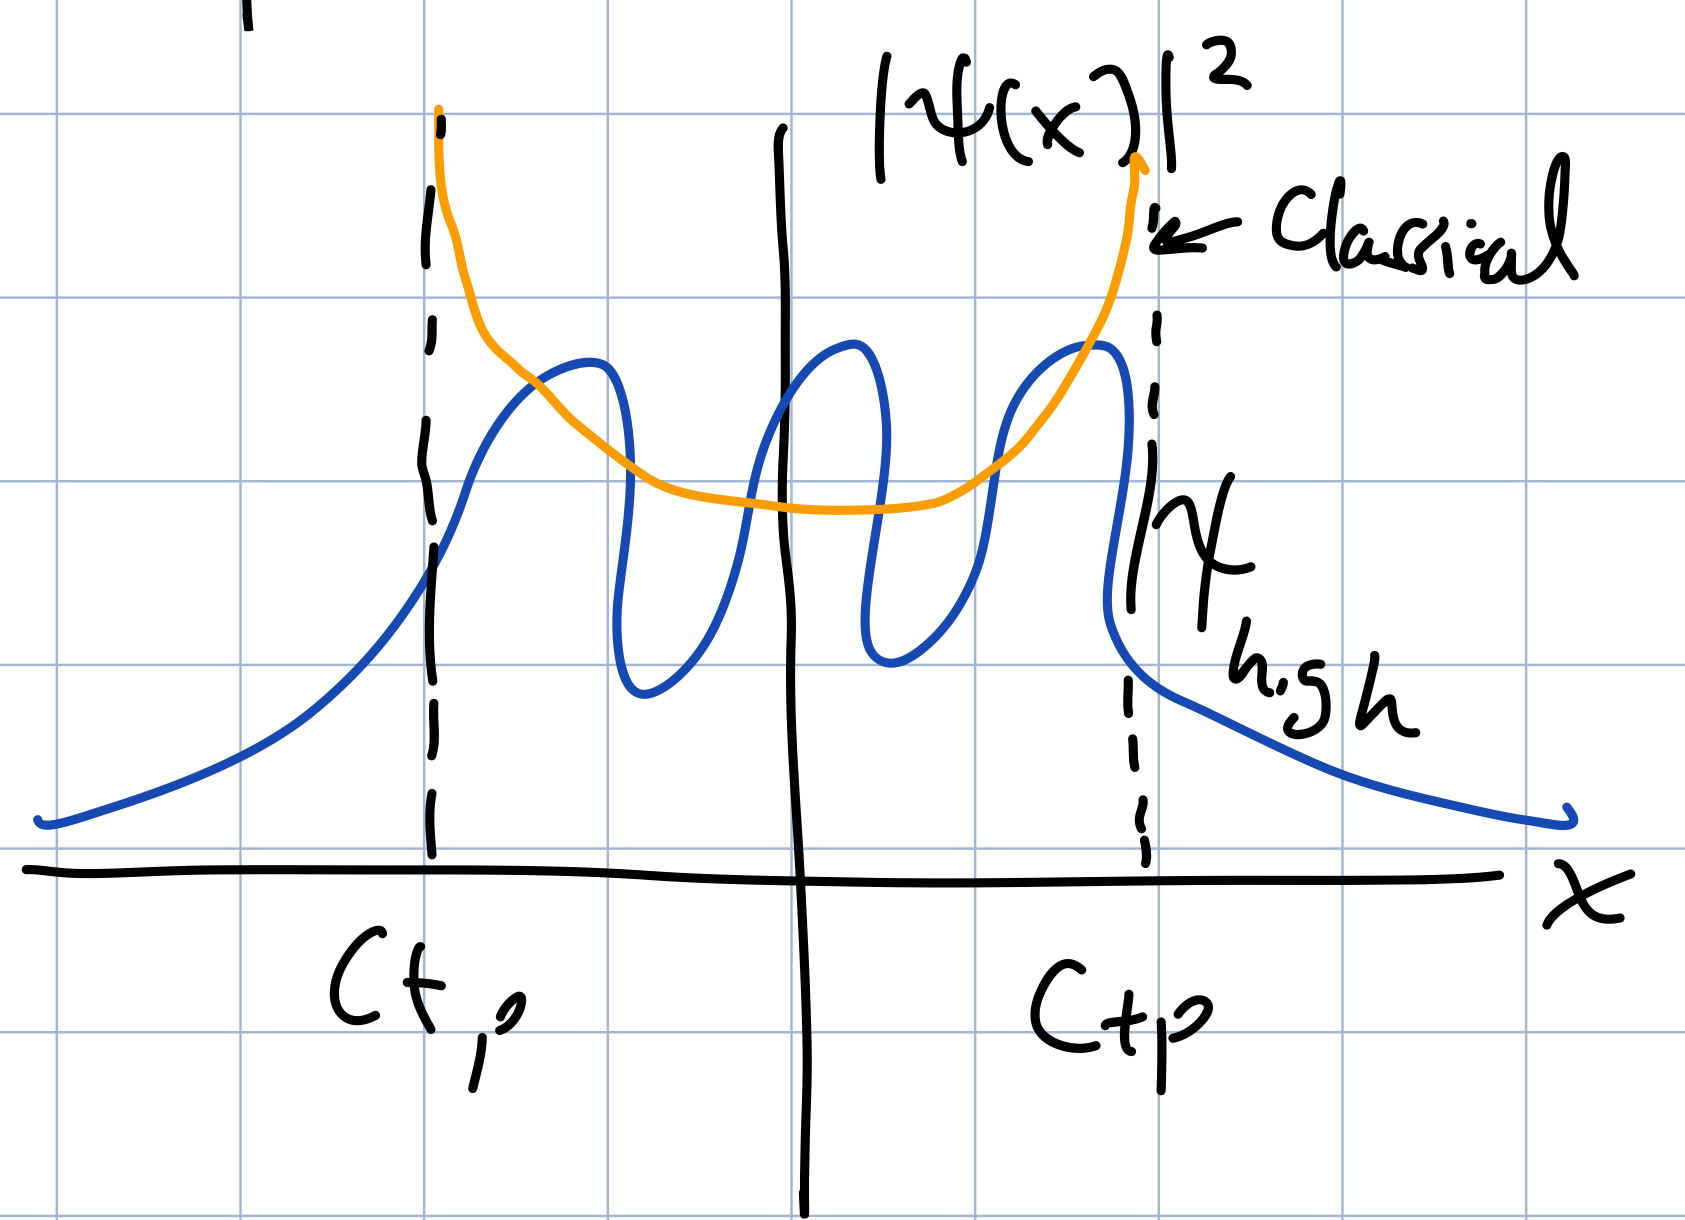
\includegraphics[width=300px]{classmis.jpeg}

\newpage
\subsection{Dirac Notation}
Now, having this wavefunction representation is really useful for plotting and visualizing the wave function.
But, we would like to do algebra on this object. So, we identify vectors and their
adjoints as:
\[ \Psi(x) \leftrightarrow \bra*{\Psi}, \Psi^*(x) \leftrightarrow \ket*{\Psi} \]
To write an inner product, we say:
\[ \braket*{\Psi}{\Psi} = \int \Psi^* \Psi \dd{x} \]
Schrodinger's equation now becomes:
\[ \hat{H} \ket*{\Psi_E} = E \ket*{\Psi_E} \]
And now to denote the expectation value, we write
\[ \langle x \rangle_{\Psi}  = \bra{\Psi}\hat{x}\ket*{\Psi}\]
\begin{definition}[Adjoint]
    The adjoint of an operator $\hat{A}$ is $\hat{A}^{\dagger}$ such that:
    \[ \langle \hat{A}x, y \rangle = \langle x, \hat{A}^{\dagger} y \rangle \]
\end{definition}
Hermitian, or self-adjoint operator corresponds to some observable
because it has real eigenvalues. 

\subsection{Revisiting the QHM}
Now, let us try to
make an operator that transitions between our QHM eigenstates. Define the state step up and down operator:
\[ \hat{a}_{\pm} = \frac{1}{\sqrt{2}} \qty[\qty(\frac{m\omega}{\hbar})^{1/2} \hat{x} \mp i \frac{\hat{p}_x}{(m\hbar \omega)^{1/2}}] \]
Note that the two operators adjoints are exactly each other.
\[ \hat{a}_{+}^{\dagger} = \hat{a}_{-} \]
Furthermore their commutator $[\hat{a}_{-}, \hat{a}_{+}] = 1$. This means
\begin{align*}
    \hat{H} &= \frac{p_x^2}{2m} + \frac{1}{2} m \omega^2 x \\
    &= \frac{\hbar \omega}{2} \qty(\hat{a}_{-} \hat{a}_{+} + \hat{a}_{+} \hat{a}_{-}) \\
    &= \hbar \omega \qty(\hat{a}_{-} \hat{a}_{+} - \frac{1}{2}) \\
    &= \hbar \omega \qty(\hat{a}_{+} \hat{a}_{-} + \frac{1}{2})
\end{align*}
This means that if we define $\hat{N} = \hat{a}_{+} \hat{a}_{-}$, it is the number operator,
which is exactly equivalent to our length Hermite derivation! Note that from the above statement, the commutator
\[ [\hat{H}, \hat{a}_{\pm}] = \pm \hbar \omega \hat{a}_{\pm} \]
What is $\hat{a}_{\pm} \ket*{E}$? Well we can act $\hat{H}$ on this, so:
\begin{align*}
    \hat{H} \hat{a}_{\pm} \ket*{E} &= \qty(\hat{a}_{\pm} \hat{H} \pm \hbar \omega \hat{a}_{\pm}) \ket*{E} \\
    &= \qty(E \pm \hbar \omega) \hat{a}_{\pm} \ket*{E}
\end{align*}
So this operator adds or subtracts a quantum of energy.